\documentclass{beamer}

\usepackage{amsmath}
\usepackage{amssymb}
\usepackage{bm}
\usepackage{hyperref}
\usepackage{csquotes}

\DeclareSymbolFont{matha}{OML}{txmi}{m}{it}% txfonts
\DeclareMathSymbol{\varv}{\mathord}{matha}{118}
\usetheme{metropolis}

%\usefonttheme{serif} % default family is serif

\setbeamertemplate{section in toc}[sections numbered]
\setbeamertemplate{subsection in toc}[subsections numbered]

\title{Article presentation :}
\subtitle{Chancel L., Rehm Y., The Carbon Footprint of Capital: Evidence from France, Germany and the US based on Distributional Environmental Accounts}
\author{COMPERAT Étienne  \\ GUGELMO CAVALHEIRO DIAS Paulo \\ ORTIZ Marie Ange}
\institute{Sciences Po}
\date{\today}

\newcommand\ReduceFont{\fontsize{10}{7.2}\selectfont}

\begin{document}

\begin{frame}
    \titlepage
\end{frame}

\begin{frame}
    \ReduceFont
    \frametitle{Outline}
    \tableofcontents[hideallsubsections]
\end{frame}

\section{Introduction}
\begin{frame}
    \tableofcontents[currentsection, hideothersubsections, sections=\value{section}]
\end{frame}

\section{Related Literature}
\begin{frame}
    \tableofcontents[currentsection, hideothersubsections, sections=\value{section}]
\end{frame}

\section{Data Sources and Methodology}
\begin{frame}
    \tableofcontents[currentsection, hideothersubsections, sections=\value{section}]
\end{frame}

\section{Carbon Footprint of the Capital}
\begin{frame}{\secname}
    \tableofcontents[currentsection, hideothersubsections, sections=\value{section}]
\end{frame}

\subsection{Capital emissions by industry and institutional sector}

\begin{frame}{\subsecname}
    \begin{columns}
        \begin{column}{0.5\textwidth}
            Industries :
                \begin{itemize}
                    \item Agriculture and mining
                    \item Energy, water and waste
                    \item Manufacturing
                    \item Transport
                    \item Real estate and construction
                    \item Health and education
                    \item Public administration
                    \item Services
                \end{itemize}
        \end{column}
        \begin{column}{0.5\textwidth}
            \ReduceFont
            Results : 
                \begin{itemize}
                    \item Manufacturing as the largest emitting sector in FR and DE
                    \item Agriculture and mining as the largest emitting sector in the US
                    \item Agriculture and mining as the most carbon-intensive sector
                    \item Similar carbon intensity for the manufacturing sector
                    \item Difference in definition for the Real Estate and Construction sector
                \end{itemize}    
        \end{column}
    \end{columns}
    \hfill \break
    Following : Table 1, Emission intensities by industry groups
\end{frame}

\begin{frame}{\subsecname}
    \begin{center}
        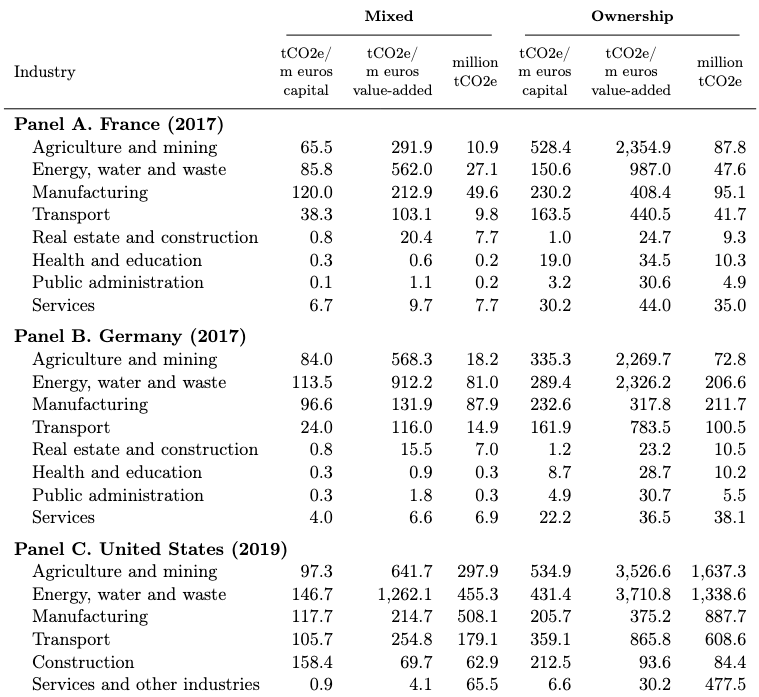
\includegraphics[height=0.9\textheight]{../Figures/T1.png}    
    \end{center}
\end{frame}

\subsection{Capital emissions by asset class}

\begin{frame}{\subsecname}
    \begin{columns}
        \begin{column}{0.5\textwidth}
            Assets :
                \begin{itemize} 
                    \item Housing assets
                    \item Business assets
                    \item Equities 
                    \item Pension assets
                    \item Fixed income assets
                \end{itemize}
        \end{column}
        \begin{column}{0.5\textwidth}
            \ReduceFont
            Results : 
                \begin{itemize}
                    \item Equity is the most polluting asset class.
                    \item Pension assets are the second most polluting asset class.
                    \item Business assets are the third most polluting asset class.
                    \item Housing has an important market valuation, but emits little.
                    \item Important intensity of pension assets for Germany.
                \end{itemize}    
        \end{column}
    \end{columns}
    \hfill \break
    In clear, there exist important differences between types of assets.
\end{frame}

\begin{frame}{\subsecname}
    \begin{center}
        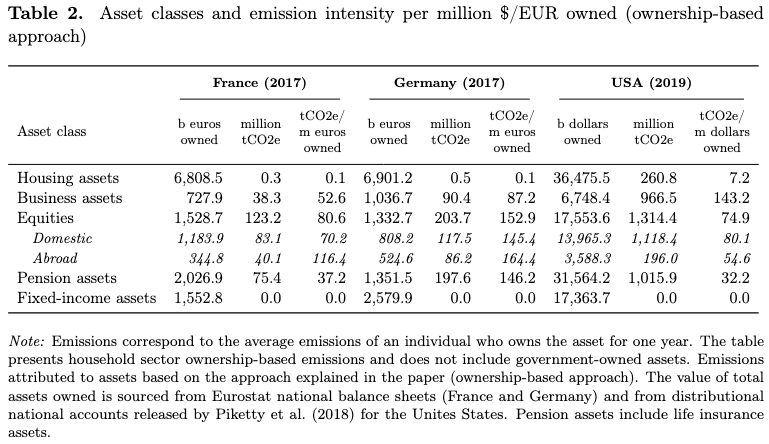
\includegraphics[width=\textwidth]{../Figures/T2.png}    
    \end{center}
\end{frame}

\subsection{The role of foreign capital in national emissions}
\begin{frame}{\subsecname}
    \begin{itemize}
        \item In France and in the US, equity held abroad represents about 20-25\% of owned equities.
        \item In Germany, equity held abroad represents about 40\% of owned equities.
        \item Foreign equity held by French and German citizens are more carbon intensive than those owned by the US citizens.
    \end{itemize}
\end{frame}

\section{The Distribution of Carbon Footprints}
\begin{frame}{\secname}
    \tableofcontents[currentsection, hideothersubsections, sections=\value{section}]
\end{frame}

\subsection{Emissions rise with income and wealth}
\begin{frame}{\subsecname}
    \begin{columns}
        \begin{column}{0.5\textwidth}
            Generally :
            \begin{itemize}
                \item Emissions are positively correlated with wealth.
                \item Consumption approach : carbon inequalities are less concentrated than income.
                \item Mixed-based approach : carbon inequalities are as concentrated as income.
                \item Ownership approach : carbon inequalities are more concentrated than wealth.
            \end{itemize}
        \end{column}
        \begin{column}{0.5\textwidth}
            \ReduceFont
            International comparison :
            \begin{itemize}
                \item The US are more carbon inequal than Germany, which is more carbon inequal than France.
                \item The majority of the US emit as much as the top of the distribution of France and Germany in the two first approaches.
                \item The top French group emits less despite owning more of the national equity than their German counterpart.
            \end{itemize}
        \end{column}
    \end{columns}
\end{frame}

\begin{frame}{\subsecname}
    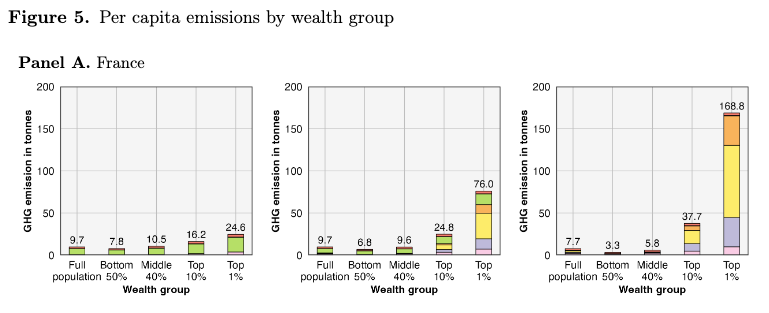
\includegraphics[width=\textwidth]{../Figures/F51.png}
\end{frame}

\begin{frame}{\subsecname}
    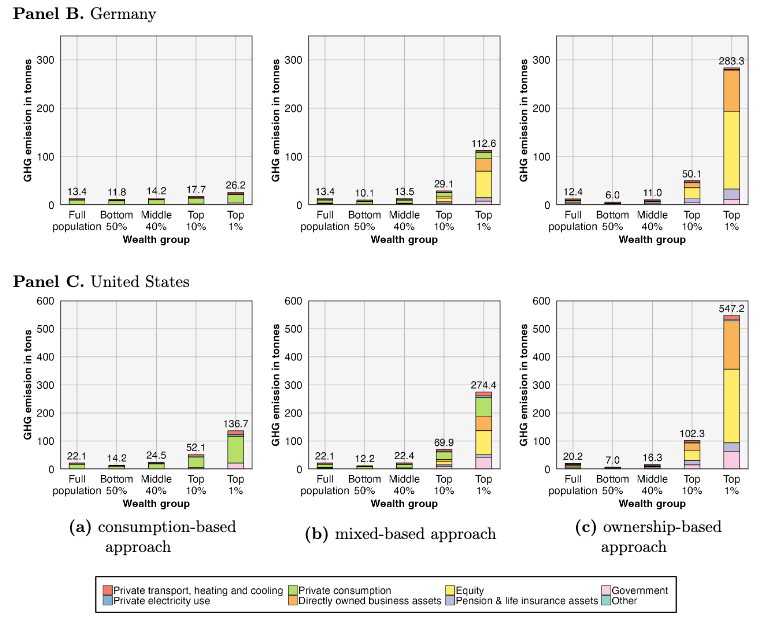
\includegraphics[width=\textwidth, height=0.9\textheight]{../Figures/F52.png}
\end{frame}

\subsection{Emissions intensity rises with wealth}
\begin{frame}{\subsecname}
    Average emission intensity tends to increase alongside with wealth at the very top of the distribution.
    This explains the greater concentration of carbon emissions compared to wealth.
    \begin{center}
        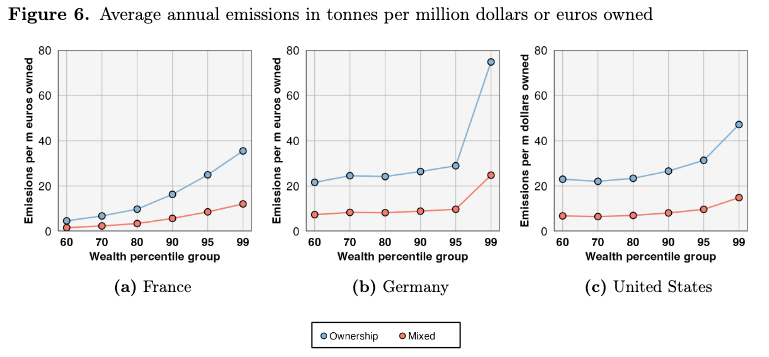
\includegraphics[width=0.9\textwidth]{../Figures/F6.png}
    \end{center}
\end{frame}

\subsection{The weight of capital emissions among top groups}

\begin{frame}{\subsecname}
    \begin{itemize}
        \item Importance of the emissions of top groups.
        \item Emissions of the top 1\% (p.36) :
        \begin{table}[!ht]
            \centering
            \begin{tabular}{|l|l|l|l|l|}
            \hline
                Countries & Consumption & Ownership & Multiplication in tCO2e \\ \hline
                France & 2.5\% & 21.5\% & 6 \\ \hline
                Germany & 2\% & 22.3\% & 11 \\ \hline
                US & 6.2\% & 26.9\% & 16 \\ \hline
            \end{tabular}
        \end{table}
        \item Key role of Capital ownership in the determinant of the top of the distribution.
        \item Structure of the emissions alongside the wealth distribution.
    \end{itemize}
\end{frame}

\begin{frame}{\subsecname}
    \begin{center}
        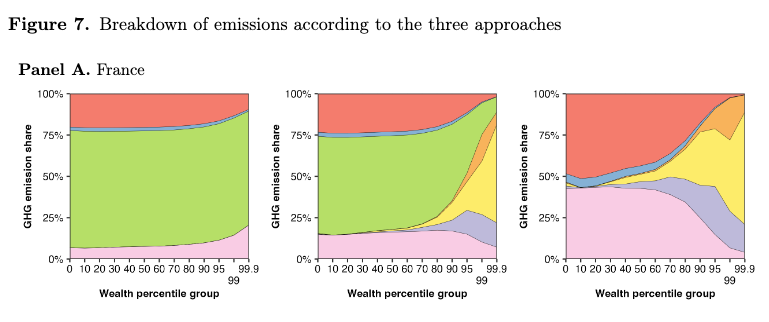
\includegraphics[width=0.9\textwidth]{../Figures/F71.png}
    \end{center}
\end{frame}

\begin{frame}{\subsecname}
    \begin{center}
        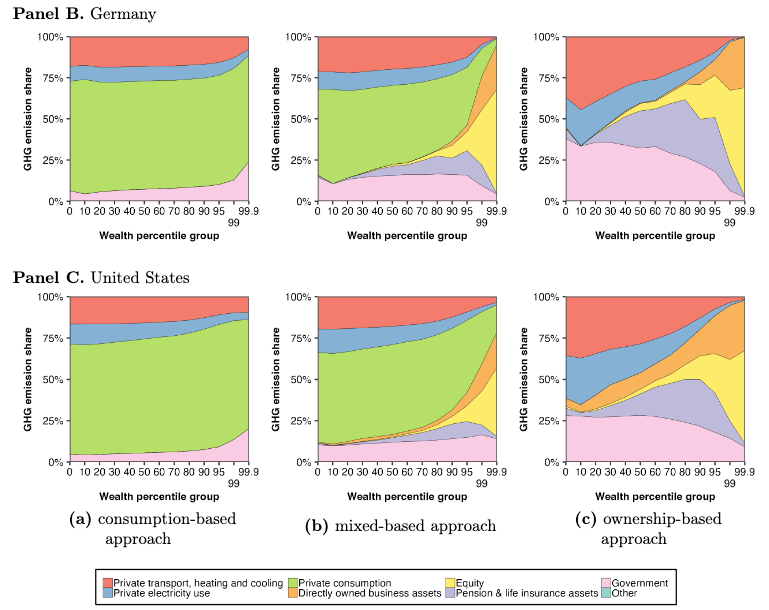
\includegraphics[width=0.9\textwidth]{../Figures/F72.png}
    \end{center}
\end{frame}

\section{Discussion}
\begin{frame}{\secname}
    \tableofcontents[currentsection, hideothersubsections, sections=\value{section}]
\end{frame}

\subsection{Sensitivity of the results to assumption}
\begin{frame}{\subsecname}
    test \\
    Include Figure 8.
    %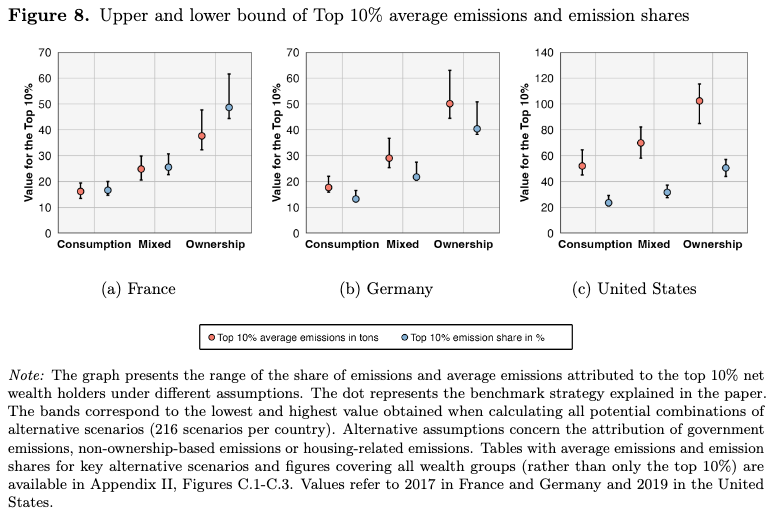
\includegraphics[width=0.9\textwidth]{../Figures/Figure_8.png}
\end{frame}

\subsection{Scope and limitations of the data and foootprinting approaches}
\begin{frame}{\subsecname}
    \begin{itemize}
        \item Limitations linked to data Sources
        \item Carbon footprints and individual responsibility
    \end{itemize}
\end{frame}

\subsection{How our estimates compare to earlier work}
\begin{frame}{\subsecname}
\end{frame}

\subsection{Stylized facts on inequality and emissions}
\begin{frame}{\subsecname}
    Stylized facts.
\end{frame}

\subsection{Distributional properties and revenue estimates for a carbon wealh tax}
\begin{frame}{\subsecname}
\end{frame}

\section{Conclusion}
\begin{frame}
    \tableofcontents[currentsection, hideothersubsections, sections=\value{section}]
\end{frame}


\end{document}